%----------------------------------------------------------------------------
\chapter{Implementation}
\label{cha:implementation}
%----------------------------------------------------------------------------

At the end of the design phase it is clearly visible, that the investigated technologies and tools what advantages have. To adopt the chosen technologies I chose to use the Java programming language. For model driven engineering the Eclipse platform serves the best tools, that's why I used Eclipse Modeling Tools to implement the application.

\begin{figure}[htp]
\centering
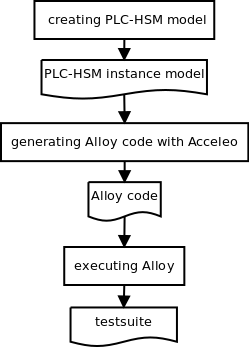
\includegraphics[scale=0.5]{figures/testgenerator_architecture}
\caption{Architecture of the test generator framework}
\label{fig:testgenerator_architecture}
\end{figure}

The test case generation process consists of the following steps (see Figure~\ref{fig:testgenerator_architecture}):

\begin{enumerate}
	\item First the instance model have to created with the default PLC-HSM model editor generated by the Eclipse Modeling Framework. The model can have all the PLC-HSM model features except the timed transitions.
	\item The next step is to create Alloy code, that can produce the test cases. The required informations can be extracted from the previously created PLC-HSM model, and so the desired Alloy code can be generated automatically. This generation was solved with Acceleo, which is a model to text transforming tool as part of the Eclipse Modeling Tools.
	
	The generated Alloy code guarantees state and transition coverages. To create the Alloy code, we need to know the name of states, transitions, their relationship, the guards and the initial state of the SUT. From these information will be the necessary Alloy signatures and predicates generated.
	\item The generated Alloy code can be executed with Alloy Analyzer to get the test suite with all the test cases.
\end{enumerate}

The generated Alloy code will be demonstrated with an example (see Figure~\ref{fig:alloy_statemachine}). The static part of the generated Alloy code can be see on Listing~\ref{lst:alloy_static}.

\begin{figure}[htp]
\centering
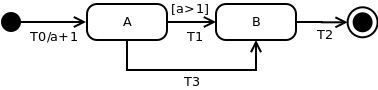
\includegraphics[scale=0.5]{figures/alloy_statemachine}
\caption{Example state machine with guard}
\label{fig:alloy_statemachine}
\end{figure}

The basic state machine element's (system, states, transitions) are between line number 4-7. The next section (line number 9-18.) describes the structure of a basic test case. One test case consists of several steps. The only given fact (line number 20-27.) defines the connection between a test case and the state machine. The predicate \texttt{inheritSystem} is a utility method, that can be used to inherit extended state variables from previous states. Predicates \texttt{transition\_coverage} and \texttt{state\_coverage} define transition and state coverage criteria accordingly. These predicates can be executed using the \texttt{run} statement used in line number 38.

\begin{lstlisting}[label={lst:alloy_static}, caption=Test suite generator Alloy code,breaklines=true]
module psm_statecoverage
open util/integer

abstract sig System {}
abstract sig State {system: one System}
abstract sig Transition {from, to: one State}
one sig Initial, End extends State {}

sig TestCase { firstStep: Step }
sig Step {
	from, to: State,
	via: Transition,
	nextStep: lone Step
} {
	via.from = from
	via.to = to
}
fun steps (tc:TestCase): set Step { tc.firstStep.*nextStep }

fact {
	all s:Step, tc:TestCase | s in tc.firstStep.*nextStep
	all tc:TestCase | tc.firstStep.from = Initial
	all t:Transition | one s:Step | s.via = t
	all curr:Step, next:curr.nextStep | next.from = curr.to
	all sys:System | some s:State | sys = s.system
	all s:State | some t:Transition | t.from = s or t.to = s
}

pred inheritSystem(s1, s2: System) { s1 = s2 }

/***** GENERATED CODE START *****/
...
/***** GENERATED CODE END *****/

pred transition_coverage() { some tc:TestCase | steps[tc].via = Transition }
pred state_coverage() { some tc:TestCase | all s:State | s in steps[tc].from + steps[tc].to }

run state_coverage for 10 but exactly 1 TestCase
\end{lstlisting}

The dynamic part of the Alloy code, generated from the instance model can be see on Listing~\ref{lst:alloy_dynamic}. The code starts with the initialization of the SUT. The structure was defined in a signature, while the initial state of the SUT needs to define in a predicate. The rest of the code describes the other parts of the state machine: the states (\texttt{A}, \texttt{B}), the transitions (\texttt{T0}, \texttt{T1}, \texttt{T2}, \texttt{T3}), the events (\texttt{E0}) and the guards (\texttt{G0}).

\begin{lstlisting}[label={lst:alloy_dynamic}, caption=Dynamically generated Alloy codes,breaklines=true]
sig S extends System { a: Int }
pred initSystem(s:System) { s.a = 0 }

one sig A, B extends State {}
lone sig T0 extends Transition {}{
	from = Initial
	to = A
	initSystem[from.system]
	E0[from.system, to.system]
}
lone sig T1 extends Transition {}{
	from = A
	to = B
	inheritSystem[from.system, to.system]
	G0[from.system]
}
lone sig T2 extends Transition {}{
	from = B
	to = End
	inheritSystem[from.system, to.system]
}
lone sig T3 extends Transition {}{
	from = A
	to = B
	inheritSystem[from.system, to.system]
}
pred E0(s1, s2: System) { s2.a = add[s1.a, 1] }
pred G0(s: System) { s.a > 1 }
\end{lstlisting}

\begin{figure}[htp]
\centering
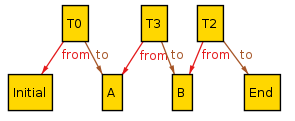
\includegraphics[scale=0.5]{figures/alloy_statecoverage}
\caption{Example test case generated from state machine in Figure~\ref{fig:alloy_statemachine}}
\label{fig:alloy_statecoverage}
\end{figure}

The above Alloy code generates test cases with state coverage guaranteed and the resulted test case is on Figure~\ref{fig:alloy_statecoverage} considering the previously defined state machine. As we can see the transition \texttt{T1}, having an unsatisfiable guard, is left out from the test case, and the generated test case satisfies all the requirements.

% chapter implementation (end)